    \subsection{Cybernetics}
        \subsubsection{Definitions}
        \subsubsection{Background}
        \subsubsection{Second-Order Cybernetics}
    \subsection{The Connection}
        \subsubsection{Design for Cybernetics}
        \subsubsection{Cybernetics for Design}
    


\section{Introduction}
	\subsection{Cybernetics: Definitions}
		\begin{frame}
%			\setbeamercovered{transparent}
			\frametitle{Definition(s) of Cybernetics}
			\framesubtitle{The Root of the Word}
			\textbf{Cybernetics} (\textbackslash \textipa{saI\texttt{}b@r"netIks}\textbackslash):
			\begin{itemize}
				\item<1-> From Greek `kybernetes': `\textcolor{teal}{steersman}'; `kybernan': `\textcolor{teal}{to steer or pilot a ship, direct as a pilot}'
				\item<2-> Having a goal and taking action to achieve that goal
				\item<3-> The art of steering \cite{pangaro_web}:
			\end{itemize}
			\centering\includegraphics<3>[width=7.2cm]{./resources/steering1.png}
			\centering\includegraphics<4>[width=7.2cm]{./resources/steering2.png}
			\centering\includegraphics<5>[width=7.2cm]{./resources/steering3.png}
			\centering\includegraphics<6>[width=7.2cm]{./resources/steering4.png}
			\centering\includegraphics<7>[width=7.2cm]{./resources/steering5.png}
			\centering\includegraphics<8>[width=7.2cm]{./resources/steering6.png}
			\centering\includegraphics<9>[width=7.2cm]{./resources/steering7.png}
			\centering\includegraphics<10>[width=7.2cm]{./resources/steering8.png}
			\centering\includegraphics<11>[width=7.2cm]{./resources/steering9.png}
			\centering\includegraphics<12>[width=7.2cm]{./resources/steering10.png}
		
%			\setbeamercovered{invisible}
		\end{frame}
		\begin{frame}
			\setbeamercovered{transparent}
			\frametitle{Definition(s) of Cybernetics (Cont'd)}
			\framesubtitle{What is?}
			\begin{itemize}
				\item<1->Ship of the State: The Command of a naval vessel is a metaphor for the governance of a city/state.\\
				--- Plato
				\item<2->``Cybernetique is the art of governing or the science of government.''\\
				--- André-Marie Ampère
				\item<3->``Use the word ‘cybernetics’, Norbert, because nobody knows what it means. This will always put you at an advantage in arguments.''\\
				Widely quoted; attributed to Claude Shannon in a letter to Norbert Wiener in the 1940s.
				\item<4->``The Science of Effective Organization''\\
				--- Stafford Beer
				\item<5->``The art and science of uderstanding.''\\
				--- Humerto Maturana
			\end{itemize}
			\setbeamercovered{invisible}
		\end{frame}
	
		\begin{frame}
			\setbeamercovered{transparent}
			\frametitle{Definition(s) of Cybernetics (Cont'd)}
			\framesubtitle{What is?}
			\begin{itemize}
				\item<1->``The art and science of manipulating defensible metaphors''
				--- Gordon Pask
				\item<2->``A form of cross-disciplinary thought which made it possible for members of many disciplines to communicate with each other easily in a language which all could understand''
				--- Margaret Mead
				\item<3->``That is the fascinating thing about cybernetics. You ask a couple of people to give you a definition and although you don’t get to know much about cybernetics from them, you find out a lot about the person supplying the definition, including their area of expertise, their relation to the world, their desire to play with metaphors, their enthusiasm for management, and their interest in communications or message theory.''\\
				--- Heinz von Foerster
			\end{itemize}
			\setbeamercovered{invisible}
		\end{frame}
	
		\begin{frame}
			\frametitle{Definition(s) of Cybernetics (Cont'd)}
			\framesubtitle{What is?}
			\begin{itemize}
				\item A clear-cut and crisp definition is very hard to find.
				\item An entire webpage is dedicated for different definitions: \url{http://asc-cybernetics.org/definitions/}\\
			\end{itemize}
		\end{frame}
	
		\begin{frame}
			\setbeamercovered{transparent}
			\frametitle{Definition(s) of Cybernetics (Cont'd)}
			\framesubtitle{Will History Help?}
			\begin{itemize}
				\item<1->The storylines do not split into distinct lines of descent.
				\item<2->The storylines do not subdivide into clear phases or stages.
				\item<3->\textcolor{red}{Cybernetics' history defies neat categories and compartments}...
				\item<4->An entire webpage and a lot of diagrams can be found about the history of Cybernetics: \url{http://www.asc-cybernetics.org/foundations/timeline.htm}
			\end{itemize}
			\setbeamercovered{invisible}
		\end{frame}
	
		\begin{frame}
			\setbeamercovered{transparent}
			\frametitle{Definition(s) of Cybernetics (Cont'd)}
			\framesubtitle{What About Ven Diagram, Set Theory, or Any Other Categoriazation Method?!}
			\begin{itemize}
				\item<1->Everybody has a different opinion as to Cybernetics' disciplinary `slot'.
				\item<2->Each person involved in Cybernetics research, draws a new line on the territory of Cybernetics. Therefore Any map of relevant people and their timeline will fail to show the exact contexts.
				\item<3->... \textcolor{red}{Cybernetics defies neat categories and compartments}
			\end{itemize}
			\setbeamercovered{invisible}
		\end{frame}
	
		\begin{frame}
			\frametitle{Definition(s) of Cybernetics (Cont'd)}
			\framesubtitle{Cybernetics defies neat categories and compartments}
			\centering
\includegraphics[height=0.7\textheight]{./resources/frustrated.png}
		\end{frame}

	\subsection{Cybernetics: Background}
		\begin{frame}
		\frametitle{Classic Examples}
		\framesubtitle{Automaticity of Behaviour in Artificial Objects}
			\begin{columns}
				\column{0.3\textwidth}
				\begin{figure}
					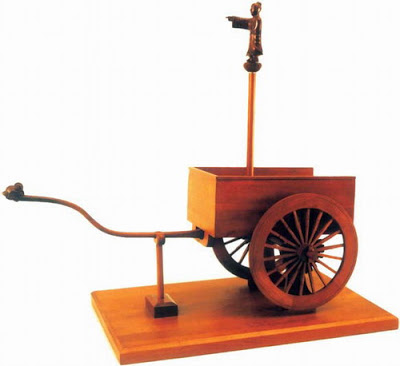
\includegraphics[width=3cm]{./resources/chinesecompasscart.jpg}
					\caption{Chinese Compass Cart}
				\end{figure}
				\column{0.3\textwidth}
				\begin{figure}
					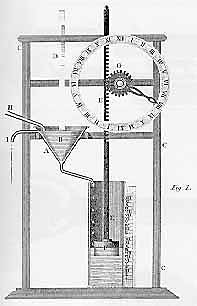
\includegraphics[width=2cm]{./resources/waterclock.jpg}
					\caption{Ctesibius's Water Clock - 300s B.C.}
				\end{figure}
				\column{0.3\textwidth}
				\begin{figure}
					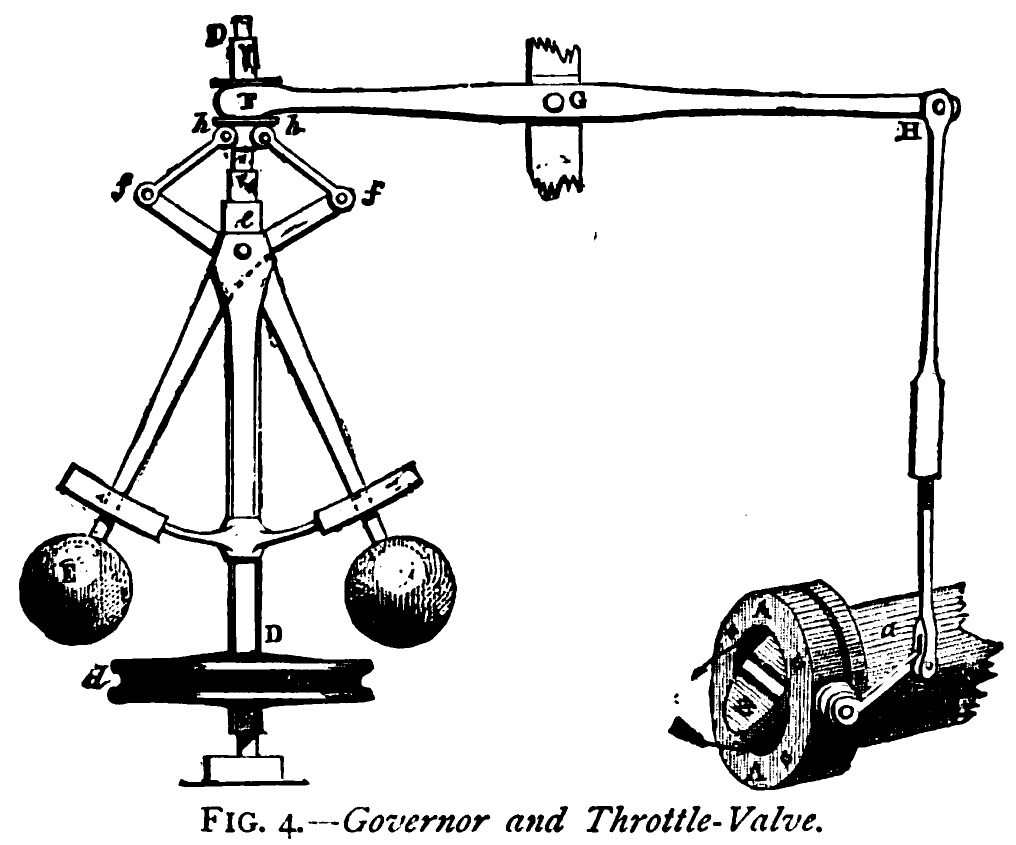
\includegraphics[width=3.5cm]{./resources/flyball.png}
					\caption{James Watt's Flyball Governor - 1780s}
				\end{figure}
			\end{columns}
			\begin{itemize}
				\item<1->All tools incorporated \textcolor{teal}{self-regulating} behavior without so much attention to a specific theory.
			\end{itemize}
		\end{frame}
		
		\begin{frame}
		\setbeamercovered{transparent}
		\frametitle{Through Systems Perspective}
		\framesubtitle{Self-Regulation Mechanisms; Machine/Organism Similarity}
			\begin{columns}
				\column{0.7\textwidth}
			        \begin{itemize}
				        \item<1->This model would remain evident in later models of \textcolor{teal}{feedback}.
				        \item<2->This model would remain evident in later models of \textcolor{teal}{feedback}.
			        \end{itemize}
				\column{0.2\textwidth}
				\begin{figure}
					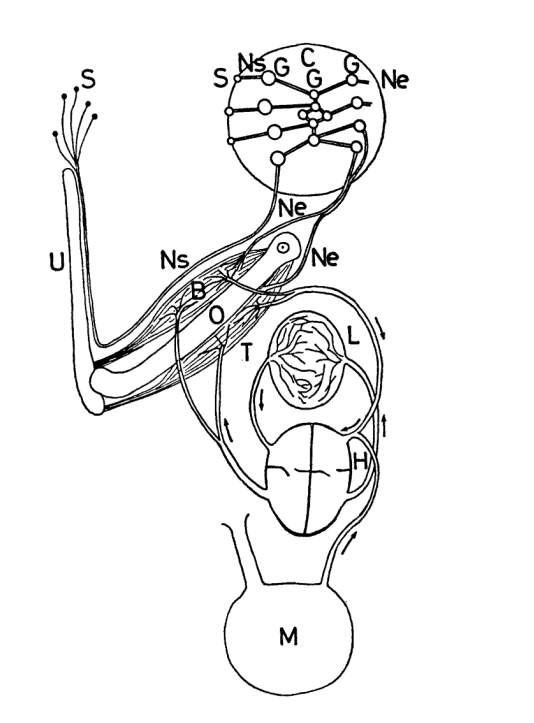
\includegraphics[width=3cm]{./resources/lincke_mechanical_relay.PNG}
				\end{figure}
			\end{columns}
		\setbeamercovered{invisible}
		\end{frame}
		
		\begin{frame}
    		\setbeamercovered{transparent}
    		\frametitle{Homeostasis}
    		\framesubtitle{Dynamic Systems' Self-Maintained Stability}
    		Introduction to Homeostasis...
    		\setbeamercovered{invisible}
		\end{frame}
		
		\begin{frame}
    		\setbeamercovered{transparent}
    		\frametitle{Teleological Implications of `Regulation'}
    		\framesubtitle{Aristotelian Dictatorship is Being Attacked!}
    		Arturo Rosenblueth (1937):\\
    		\begin{columns}
    		    \column{0.7\textwidth}
    		        \begin{itemize}
    		            \item<1->Regulation $\longrightarrow$ Prospective \textcolor{teal}{goal} or \textcolor{teal}{purpose}
    		            \item<2->Purposeful behaviour:
    		                \begin{itemize}
    		                    \item Feed-back (teleological): positive or negative
    		                    \item Non-feed-back (non-teleological)
    		                \end{itemize}
		                \item<3->All purposeful behaviour must require negative feed-back
		                \item<4->Purposefulness is independent of causality, effective or final
    		        \end{itemize}
    		    \column{0.3\textwidth}
    		        \begin{figure}
					    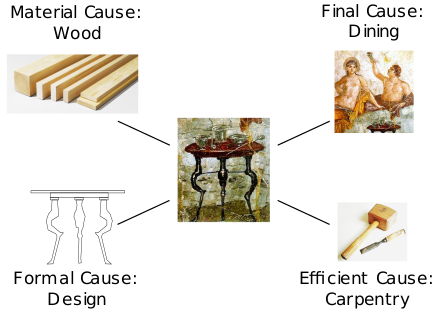
\includegraphics[width=3cm]{./resources/4cause.png}
				    \end{figure}
    		\end{columns}
    		\setbeamercovered{invisible}
		\end{frame}
	\subsection{Cybernetics of Cybernetics: Second Order}
		\begin{frame}
		\end{frame}
	\subsection{Design}